% !TEX program=pdflatex
% LaTeX rebuttal letter example. 
% 
% Copyright 2019 Friedemann Zenke, fzenke.net
%
% Based on examples by Dirk Eddelbuettel, Fran and others from 
% https://tex.stackexchange.com/questions/2317/latex-style-or-macro-for-detailed-response-to-referee-report
% 
% Licensed under cc by-sa 3.0 with attribution required.

\documentclass[12pt]{article}
\usepackage[utf8]{inputenc}
\usepackage{lipsum} % to generate some filler text
\usepackage{fullpage}
\usepackage{times}
\usepackage{amsmath, amsthm, amsfonts}
\usepackage{booktabs}
\usepackage{makecell}
\usepackage{multirow}
\usepackage{lscape}
\usepackage{xcolor}
\usepackage{float}
\usepackage{subfig}
\usepackage{graphicx}
\usepackage{framed}
\usepackage{soul}
\usepackage[colorlinks=true, linkcolor=blue, citecolor=black]{hyperref}
\usepackage{natbib}
% Vector
\newcommand{\MyVec}[1]{\boldsymbol{#1}}
% Matrix
\newcommand{\MyMat}[1]{\boldsymbol{#1}}
% Vectors with hat
\newcommand{\hvec}[1]{\hat{\boldsymbol{h}}_{#1}}
% Model parameters
\newcommand{\Param}[1]{\textcolor{blue}{#1}}

\usepackage{blindtext}
\usepackage[most]{tcolorbox} 
\definecolor{block-gray}{gray}{0.95}


\newtcolorbox{zitat}[2][]{%
    colback=block-gray,
    grow to right by=-0mm,
    grow to left by=-0mm, 
    boxrule=0pt,
    boxsep=0pt,
    breakable,
    enhanced jigsaw,
    borderline west={4pt}{0pt}{gray},
    title={#2\par},
    colbacktitle={block-gray},
    coltitle={black},
    fonttitle={\bfseries},
    attach title to upper={},
    #1,
}

\newenvironment{myquote}[1]%
{\vspace{0.5em}\begin{zitat}{#1}}
{\end{zitat}\vspace{0.5em}}


% import Eq and Section references from the main manuscript where needed
% \usepackage{xr}
% \externaldocument{manuscript}

% package needed for optional arguments
\usepackage{xifthen}
% define counters for reviewers and their points
\newcounter{reviewer}
\setcounter{reviewer}{0}
\newcounter{point}[reviewer]
\setcounter{point}{0}

% This refines the format of how the reviewer/point reference will appear.
\renewcommand{\thepoint}{P\,\thereviewer.\arabic{point}} 

% command declarations for reviewer points and our responses
\newcommand{\reviewersection}{\stepcounter{reviewer} \bigskip \hrule \setcounter{figure}{0}\section*{Reviewer \thereviewer}}

\newenvironment{point}
   {\refstepcounter{point} \bigskip \noindent {\textbf{Reviewer~Point~\thepoint} } ---\ \begin{sf}}
   {\end{sf} \par}

\newcommand{\shortpoint}[1]{\refstepcounter{point}  \bigskip \noindent 
	{\textbf{Reviewer~Point~\thepoint} } ---\begin{sf} ~#1 \end{sf}\par}

\newenvironment{reply}
   {\medskip \noindent \textbf{Reply}:\  }
   {\medskip}

\newcommand{\shortreply}[2][]{\medskip \noindent \textbf{Reply}:\  #2
	\ifthenelse{\equal{#1}{}}{}{ \hfill \footnotesize (#1)}%
	\medskip}

% Numbering figures according to reviewers
\renewcommand{\thefigure}{\thereviewer{}-\arabic{figure}}

\begin{document}

\section*{Response to the Reviewers}
% General intro text goes here
We thank the reviewers for their critical assessment and insightful comments on our work.
%
We have made extensive modifications to our manuscript, including adding more experiments and improving the presentation.
%
In the following, we first summarize the major changes we made.
%
%We also prepare an \emph{annotated version} for our revised manuscript.
%
%In the annotated version, changes corresponding to each point are all highlighted by red squares.

\subsection*{Summary of Changes}

\begin{enumerate}
\item According to reviewer 1's comments, we have added experiments on the performance bottleneck analysis of GNN inference.
%
Specifically, we added experiments on how the hyper-parameters of GNNs affect the elapsed time and the memory usage of inference in Section 4.1.2 ``Effects on Inference Time'' and Section 4.1.3 ``Effects on Peak Memory Usage'', respectively.
%
We presented the time breakdown analysis of GNN inference in Section 4.2.4.
%
We also presented the memory usage analysis of GNN inference in Section 4.3, and the performance bottlenecks of the sample-based inference were analyzed in Section 4.4.3.

\item According to reviewer 2's comments, we have added an evaluation of how the model complexity and the sampling techniques affect the accuracy of GNNs.
%
Specifically, we evaluated the effects of hyper-parameters of GNNs on accuracy in Section 4.1.4.
%
We also compared the accuracy of the four typical GNNs in that section.
%
Finally, we analyzed the effects of the sampling techniques on accuracy in Section 4.4.4.

\item We have adjusted the abstract, Section 1 ``Introduction'', Section 5 ``Insights'', and Section 7 ``Conclusion'' according to the new findings on inference time and accuracy.

\item We have polished the presentation of our manuscript.
%
We unified the symbol usage through the manuscript and added a table to summarize the frequently-used symbols as suggested by reviewer 1.
%
We improved the description of the sub-layer concept in Section 2.2 and Section 2.3.
%
We also replotted some figures to improve readability.


\end{enumerate}

We then respond to the concerns of all reviewers point by point as follows.


% Let's start point-by-point with Reviewer 1
\reviewersection

% R1Q0
\begin{point}
    The authors conduct an empirical analysis of performance bottlenecks in graph neural network training. The authors identify the edge-related calculation is the performance bottleneck. Experimental of several GNN variants, such as GCN, GGNNNN, GAT and GaAN on six real-world graph datasets verify the importance of the findings. The experimental analysis is sufficient. However, there are some tiny issues in this paper.
\end{point}

\begin{reply}
    Thank you for your comments on our manuscript.
    %
    We have revised the manuscript according to your suggestions. 
    %
    Please see the replies below.
\end{reply}

% R1Q1
\begin{point}
	There are lots of symbols in this paper. Some symbols are reused and confusing, such as s denotes sub-layers or edge features.
\end{point}

% Our reply
\begin{reply}
    We apologize for the confusing use of symbols.
    %
    To clarify the symbol usage, we have unified the usage of symbols in the revised manuscript.
    %
    After revision, each symbol only represents one meaning.
    
    Specifically, we use $\boldsymbol{s}$ to represent aggregated vectors in graph neurons.
    %
    We use $\boldsymbol{s}^l_x$ to denote the aggregated vector of the graph neuron corresponding to the vertex $v_x$ in the GNN layer $l$.
    %
    If the GNN layer $l$ has sub-layers, $\boldsymbol{s}^{l,i}_x$ represents the aggregated vector of $v_x$ in the $i$-th sub-layer.
    %
    As for edges and their feature vectors, we use $e_{y,x}$ to represent an edge pointing from $v_y$ to $v_x$ and we use $\boldsymbol{e}_{y,x}$ to represent its feature vector.
    
    To facilitate readers to quickly locate the meaning of symbols, we have added Table 1 at the beginning of Section 2 ``Review of Graph Neural Networks'' in the revised manuscript.
    
%    \begin{table}[H]
%        \footnotesize
%        \caption{Frequently-used Symbols}
%        \label{tab:symbols}
%        \centering
%        \begin{tabular}{p{3em}lp{35em}}
%            \toprule
%            Category & Symbol & Meaning \\
%            \midrule
%            \multirow[c]{4}{3em}{Graph Structure}& $\mathcal{G}=(\mathcal{V}, \mathcal{E})$ & The simple undirected input graph with the vertex set $\mathcal{V}$ and the edge set $\mathcal{E}$. \\
%            & $v_x$ & The $x$-th vertex of the input graph. \\
%            & $e_{y,x}$ & The edge pointing from $v_y$ to $v_x$ of the input graph. \\
%            & $\mathcal{N}(v_x)$ & The adjacency set of $v_x$ in the input graph. \\ 
%            & $\bar{d}$ & The average degree of the input graph. \\ \midrule
%            \multirow[c]{6}{3em}{GNN Definition}& $L$ & The number of GNN layers. \\
%            & $K$ & The number of heads in a GNN layer. \\
%            & $\phi^l$ & The messaging function of the GNN layer $l$. \\
%            & $\Sigma^l$ & The aggregation function of the GNN layer $l$. \\
%            & $\gamma^l$ & The vertex updating function of the GNN layer $l$. \\ 
%            & $\phi^{l,i}$ / $\Sigma^{l,i}$ / $\gamma^{l,i}$ & The messaging/aggregation/updating function of the $i$-th sub-layer of the GNN layer  $l$.\\
%            & $\textcolor{blue}{\boldsymbol{W}^l, \boldsymbol{W}^{(k)}/\boldsymbol{b}, \boldsymbol{a}}$ & The matrices/vectors represented by the blue characters are the weight matrices/vectors that need to be learned in the GNN. \\  \midrule
%            \multirow[c]{8}{3em}{Vector}& $\boldsymbol{v}_x$ & The feature vector of the vertex $v_x$. \\
%            & $\boldsymbol{e}_{y,x}$ & The feature vector of the edge $e_{y,x}$.  \\
%            & $\boldsymbol{h}_x^{l}$ &  The {input} hidden vector of the graph neuron corresponding to $v_x$ in the GNN layer $l$. \\
%            & $\boldsymbol{h}_x^{l+1}$ &  The {output} hidden vector of the graph neuron corresponding to $v_x$ in the GNN layer $l$.\\
%            & $\boldsymbol{m}_{y,x}^l$ & The message vector of the edge $e_{y,x}$ outputted by $\phi^l$ of the GNN layer $l$. \\
%            & $\boldsymbol{s}_{x}^l$ & The aggregated vector of the vertex $v_x$ outputted by $\Sigma^l$ of the GNN layer $l$. \\
%            & $\boldsymbol{h}_{x}^{l,i}$ / $\boldsymbol{m}_{y,x}^{l,i}$ / $\boldsymbol{s}_{x}^{l,i}$ & The hidden/message/aggregated vector of the vertex $v_x$ outputted by $\gamma^{l,i}$/$\phi^{l,i}$/$\Sigma^{l,i}$ of the $i$-th sub-layer of the GNN layer $l$. \\
%            & $d^l_{in}$, $d^l_{out}$ &  The dimension of the input/output hidden vectors of the GNN layer $l$. \\
%            & $dim(\MyVec{x})$ & The dimension of a vector $\MyVec{x}$. \\
%            \bottomrule
%        \end{tabular}
%\end{table}

\end{reply}

% R1Q2
\begin{point}
    Some typical applications of GNNs should be included, such as video object segmentation [ref1], human-object interaction [ref2] and human-parsing [ref3].[1] Zero-shot video object segmentation via attentive graph neural networks,iccv 2019 [2] Learning human-object interactions by graph parsing neural networks, eccv 2018. [3] Hierarchical human parsing with typed part-relation reasoning, cvpr 2020.
\end{point}

\begin{reply}
	Thank you for pointing out the missing references. Computer vision is indeed an important application area of graph neural networks. We have added the mentioned references in Section 1 ``Introduction'' in the revised manuscript.
\end{reply}

% R1Q3
\begin{point}
There are some grammar errors and typos:
\\
  - `Take the demo GNN in Figure 1(a) as  the example.'
\\
 - `to calculate the  output hidden vector $h^{l+1}$ of the current layer l, i.e., $h^{l+1}$ = $\gamma^l(h^l,s^l)$ The end-to-end training requires…'
\\
 - `Implementing it with the specially optimized basic operators on the GPU is a potential optimization'
\\
 - The sentences in the experimental section should be unified.
\end{point}

\begin{reply}

    Thank you for pointing them out.
    %
    We feel sorry for our carelessness.
    %
    We have proofread our revised manuscript to eliminate grammar errors and typos.
    %
    We have also unified the tenses of the sentences in Section 3 ``Evaluation Design'' and Section 4 ``Evaluation Results and Analysis''.
    %
    Specifically, we use the past tense to describe experimental methods, results, and what they indicate.
    %
    We use the present tense in the sentences that FigureX or Table X is the subject of the sentences.

\end{reply}

% R1Q4
\begin{point}
    Figures 6 and 7 should be adjusted. The figures and fonts are too small.
\end{point}

\begin{reply}
    
    As suggested, we have split Figure 6 into four figures (Figure 6 to 9) in the revised manuscript to enlarge their subfigures.
    %
    Besides Figure 6 and Figure 7, we have also adjusted font sizes in all figures to make them equal to or greater than the font size of figure captions.    
\end{reply}

% R1Q5
\begin{point}
    In my view, computation efficiency is to describe the testing or validation process. Except for reporting and analyzing the training times, it is meaningful to discuss the inference time. This is also an important point of view for deep learning researchers to be concerned about.
\end{point}

\begin{reply}
    Thank you for the insightful comment and suggestion.
    %
    The efficiency of inference (including inference time and memory usage) is indeed important for deep learning researchers and engineers.
    %
    We add a brief description of GNN inference in Section 2.5 ``Inference with GNNs'' in the revised manuscript.
    %
    As suggested, we also use the same methodology as the training phase to analyze the performance bottlenecks in the inference phase.
    %
    We add corresponding experimental results in every subsection of Section 4 ``Evaluation Results and Analysis.''
    %
    \begin{enumerate}
    
    \item In Section 4.1 ``Effects of Hyper-parameters on Performance'', we conduct extra experiments on how the hyper-parameters of GNNs affect the time and peak memory usage of inference.
    %
    We find that the effects of hyper-parameters on the inference time and memory usage are the same as the training time.
    %
    When the other hyper-parameters are fixed, each hyper-parameter itself affects the training time and memory usage in a linear way.
    %
    The complexity analysis of GNNs holds for both training and inference.
    %
    We present specific experimental results in Section 4.1.2 ``Effects on Inference Time'' and Section 4.1.3 ``Effects on Peak Memory Usage'' in the revised manuscript.
    
    \item In Section 4.2 ``Time Breakdown Analysis'', we additionally conduct time breakdown analysis for GNN inference and compare the similarities and differences between training and inference.
    %
    As for the similarities, we find that the performance characteristics of inference and training are highly similar on the layer level and the step level of edge calculation.
    %
    The edge calculation stage is the main performance bottleneck for both training and inference.
    %
    %The specific performance bottlenecks of the edge calculation stage depend on the time complexity of the messaging function $\phi$ of the GNN.
    %
    As for the differences, training and inference are different mainly in two aspects: the elapsed time and the top time-consuming basic operators.
    %
    The inference time is much less than the training time.
    %
    The top time-consuming basic operators used in the backward phase of training are replaced by the basic operators used in the prediction layer of inference.
    %
    The inference time is 34\% (GCN), 32\% (GGNN), 25\% (GAT), and 32\% (GaAN) of the training time on average, as shown in Figure~\ref{fig:compare_wall_clock_time_of_training_and_inference}.
    %
    Since the inference only conducted the forward propagation from the input layer to the prediction layer, the inference time is very close to the time of the forward phase in training.
    %
    For the top time-consuming basic operators, some top operators from the backward phase in training are replaced by operators from the prediction layer in inference.
    %
    For example, Figure~\ref{fig:compare_top_basic_operators} shows that the \texttt{gather} operator used in the backward phase of training is replaced by the \texttt{index} operator used in the prediction layer of GCN.
    %
    Though the top time-consuming basic operators are changed, they still indicate that GPUs are suitable for conducting GNN inference.
    %
    We present more details of time breakdown analysis on GNN inference in Section 4.2.4 ``Performance Bottlenecks in Inference'' in the revised manuscript.
        
    \begin{figure}[h]
        \centering
        \subfloat[\texttt{amc}]{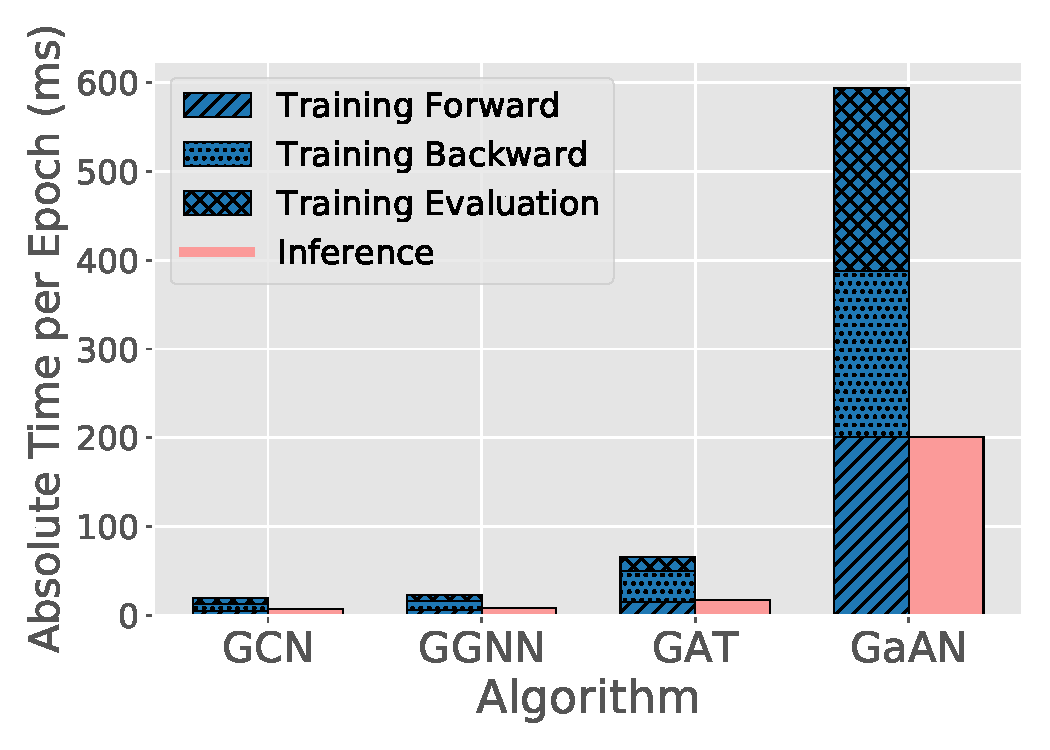
\includegraphics[width=0.33\columnwidth]{../figs/experiments/exp_time_comparison_between_training_inference_amazon-computers.pdf}}
        \subfloat[\texttt{amp}]{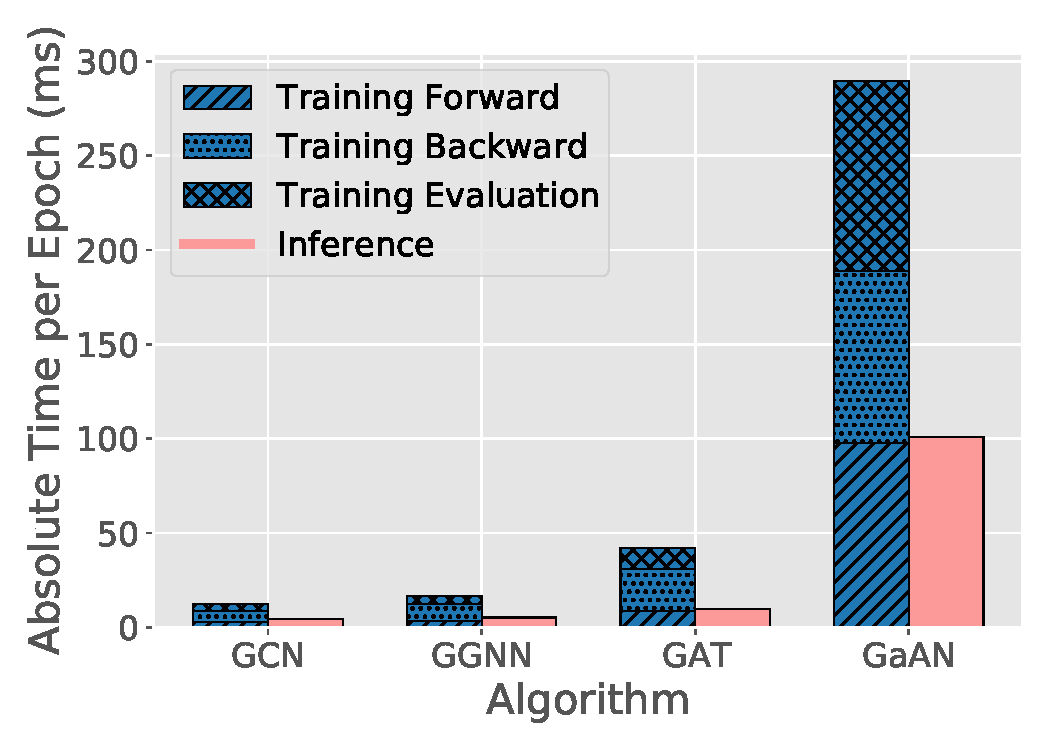
\includegraphics[width=0.33\columnwidth]{../figs/experiments/exp_time_comparison_between_training_inference_amazon-photo.pdf}}
        \subfloat[\texttt{fli}]{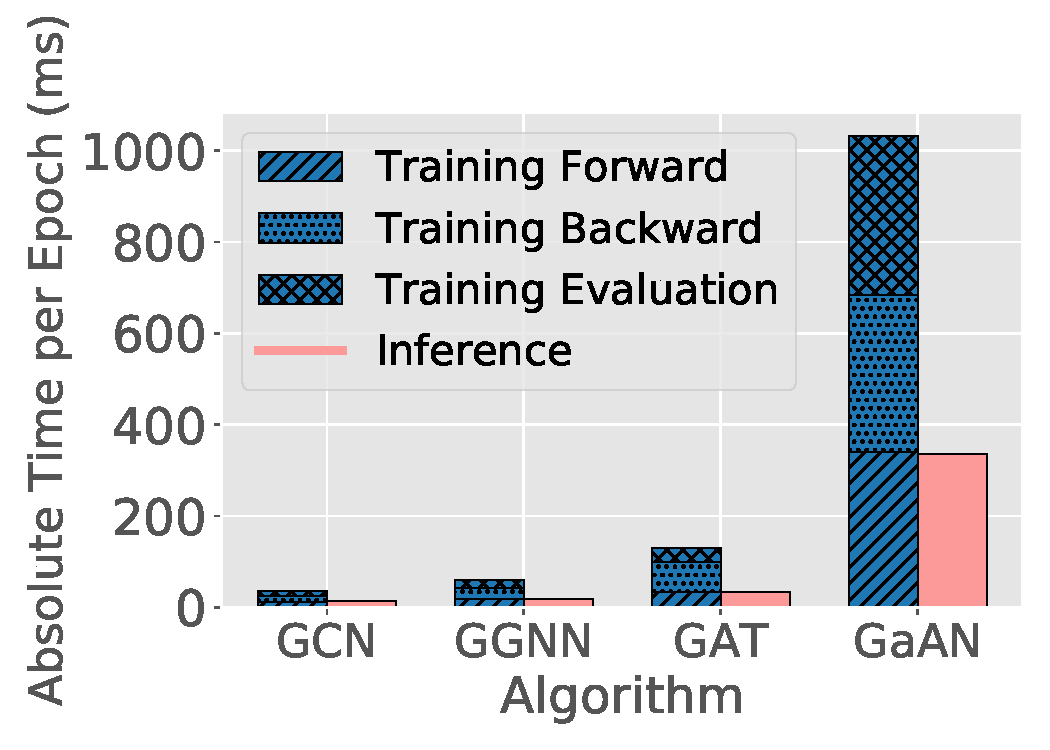
\includegraphics[width=0.33\columnwidth]{../figs/experiments/exp_time_comparison_between_training_inference_flickr.pdf}}
        \caption{Comparison of wall-clock training time and inference time on different datasets.}
        \label{fig:compare_wall_clock_time_of_training_and_inference}
    \end{figure}
    
    \begin{figure}[h]
        \centering
        \subfloat[Training]{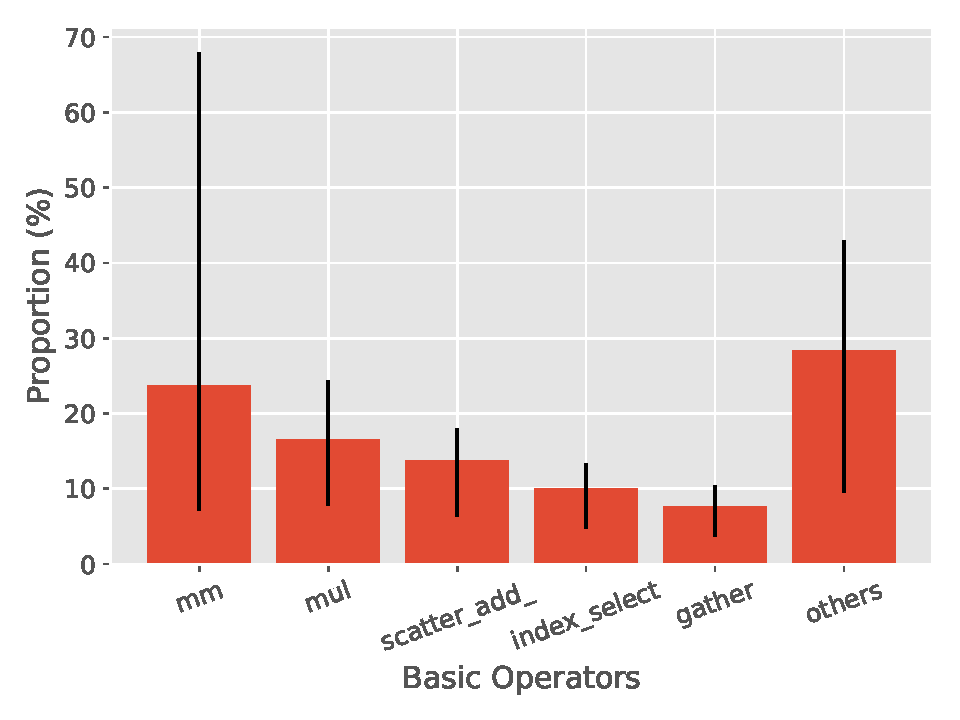
\includegraphics[width=0.4\columnwidth]{../figs/experiments/exp_top_basic_ops_gcn.pdf}}
        \subfloat[Inference]{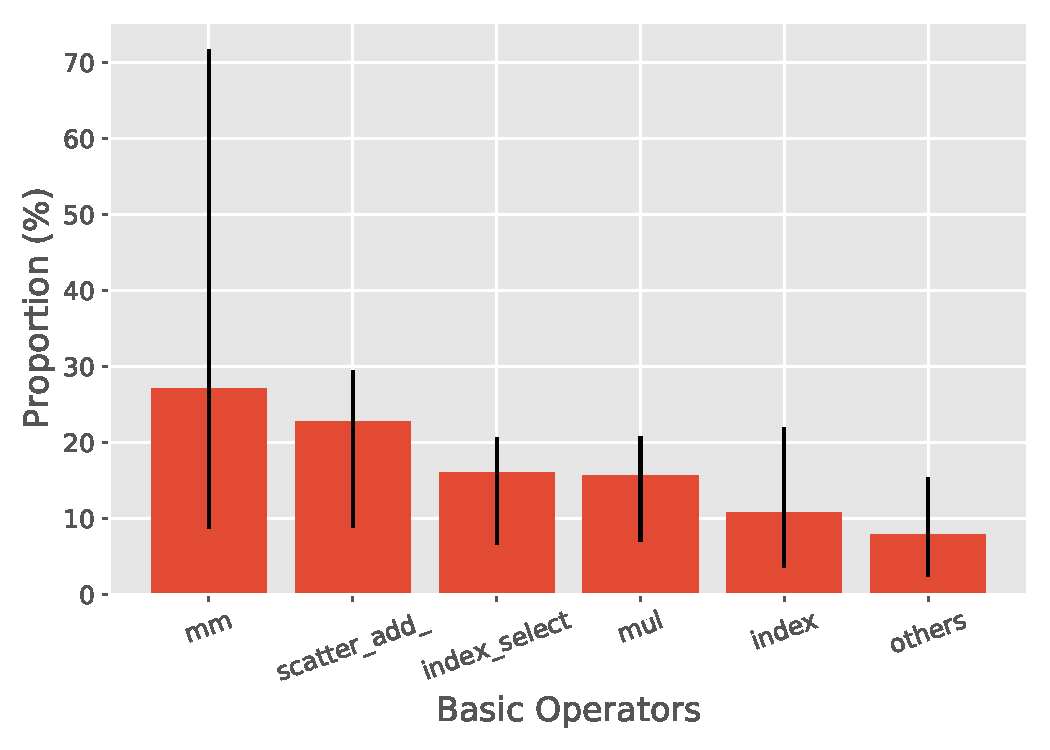
\includegraphics[width=0.4\columnwidth]{../figs/experiments/exp_inference_full_top_basic_ops_gcn.pdf}}
        \caption{Top 5 time-consuming basic operators of GCN. The time proportion of each basic operator is averaged over all datasets with the error bar indicating the maximum and the minimum.}
        \label{fig:compare_top_basic_operators}
    \end{figure}
    
    \item In Section 4.3 ``Memory Usage Analysis'', we conduct a group of experiments to evaluate the peak memory usage during inference.
    %
    We find that the memory usage of inference also mainly comes from the edge calculation stage, the same as training.
    %
    However, the memory expansion ratios of inference are much less than training.
    %
    The memory expansion ratios of inference are 45\% to 83\% (GGNN), 52\% to 61\% (GAT), and 37\% to 69\% (GaAN) of training, as indicated by Figure~\ref{fig:compare_memory_expasion_ratio}.
    %
    GGNN, GAT, and GaAN have to cache some intermediate results during training, the memory space of those results is saved during inference.
    %
    However, the memory expansion ratios of inference are still high, preventing us from performing inference on big graphs.
    %
    More details are available in Section 4.3 ``Memory Usage of Inference'' in the revised manuscript.
    
    \begin{figure}[h]
        \subfloat[Training]{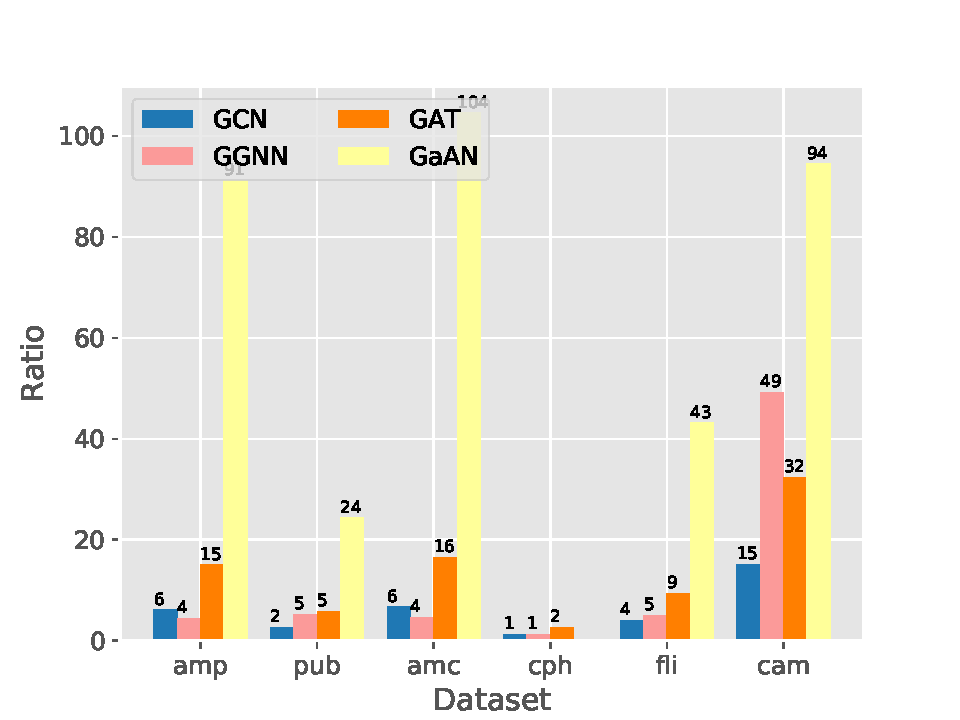
\includegraphics[width=0.5\columnwidth]{../figs/experiments/exp_memory_expansion_ratio.pdf}}
        \subfloat[Inference]{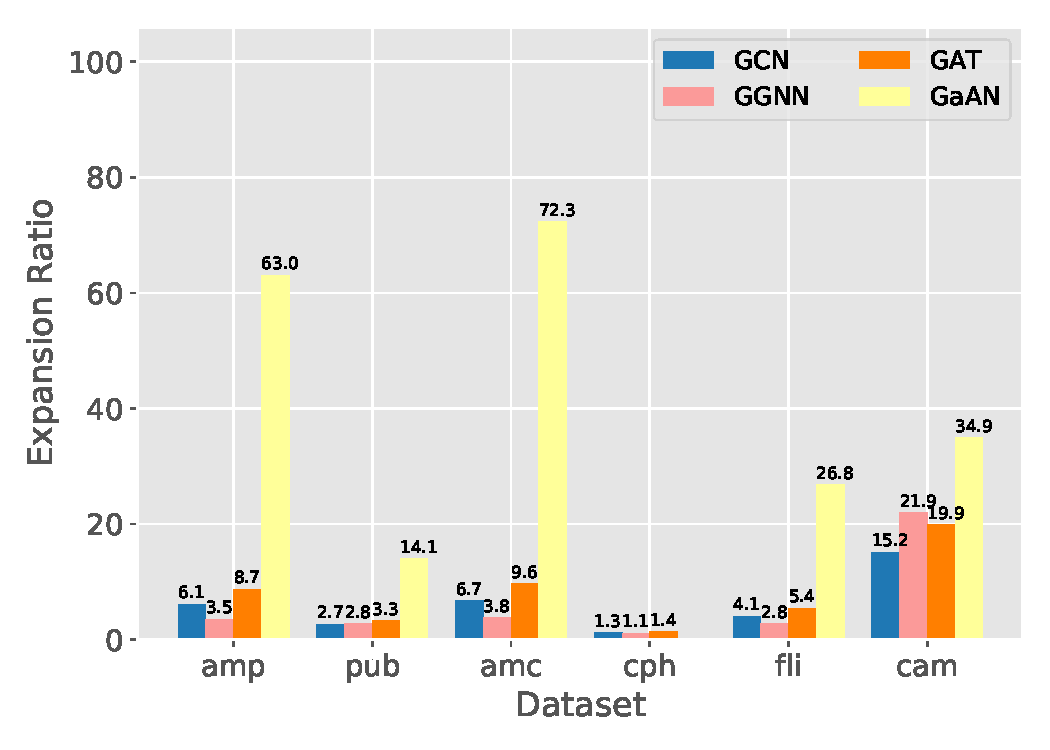
\includegraphics[width=0.5\columnwidth]{../figs/experiments/exp_inference_full_memory_expansion_ratio.pdf}}
        \caption{Memory expansion ratios of typical GNNs.}
        \label{fig:compare_memory_expasion_ratio}
    \end{figure}
    
    \item In Section 4.4 ``Effects of Sampling Techniques on Performance'', we additionally conduct experiments to analyze performance bottlenecks in sample-based inference.
    %
    We find that the batch size used in inference should be smaller than training to avoid the out of memory exception on the GPU side.
    %
    The current implementation of the inference sampler in PyG is still inefficient.
    %
    The overheads of sampling and data transferring are significant in the total inference time.
    %
    Under the same batch size, we find that the subgraph sampler used in inference tends to produce larger subgraphs than the neighbor sampler used in training.
    %
    Thus, the batch size must be small to avoid the out of memory exception on the GPU side.
    %
    At the same time, the overheads brought by sampling and data transferring from CPU to GPU become obvious when the batch size was small.
    %
    They account for near half of the total inference time on the \texttt{amp} and \texttt{cam} datasets, as shown in Figure~\ref{fig:time_breakdown_of_inference_sampler}.
    %
    We present more details of our experimental analysis in Section 4.4.3 ``Performance Bottlenecks in Inference'' in the revised manuscript.

     \begin{figure}[h]
            \centering           
            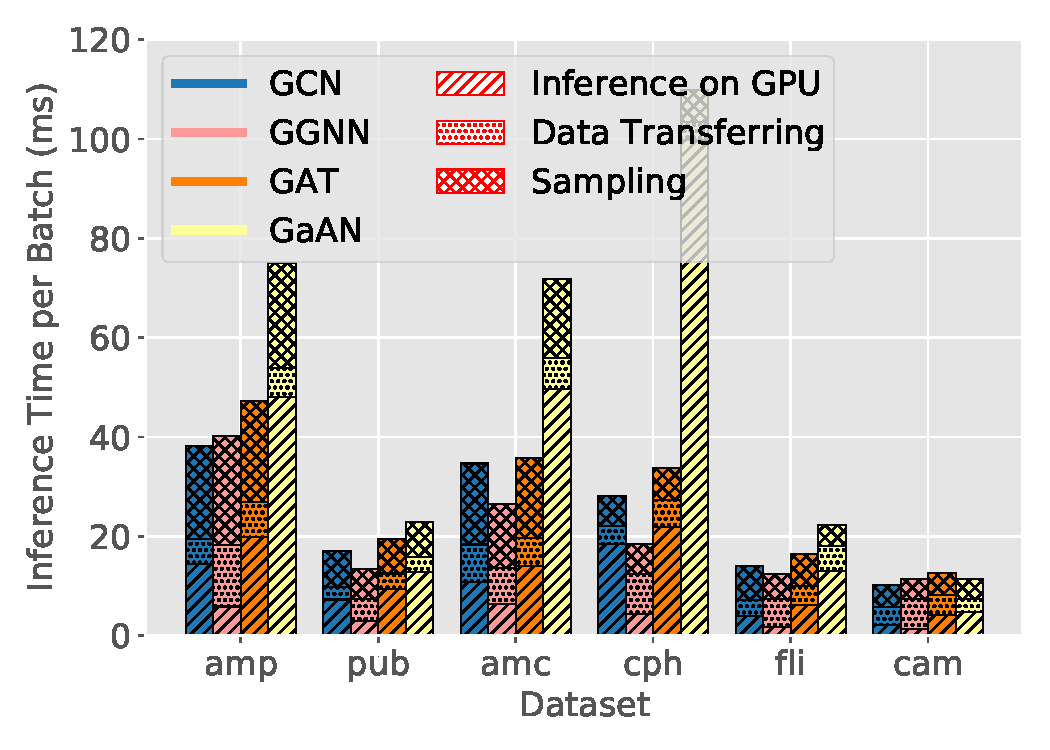
\includegraphics[width=0.5\columnwidth]{../figs/experiments/exp_inference_sampling_fix_batch_size_train_time_stack_2048.pdf}
            \caption{Inference time per batch breakdown under the batch size of 2048.}
            \label{fig:time_breakdown_of_inference_sampler}
    \end{figure}
    
    \end{enumerate}
    
\end{reply}

% Begin a new reviewer section
\reviewersection

\begin{point}
    In the paper, authors accomplished a unique study and analysis on GNN models training complexity.  The articles first review and development history of GNNs and creatively model all architectures as input layers, intermediate layers of graph neurons and prediction layers. And they quantitatively summarize the time and space complexity of 4 representative GNNs, including graph convolution, gated recurrent graph net, graph attention net and GraphSage. Most importantly, the article first break down complexity into operator level and offered analysis of good granularity, giving reader more guidance in future study. At last, the solid experiments included the study of effects of hyper-parameters and a comparison of two major sampling techniques: neighbor sampling and cluster sampling.
\end{point}

\begin{reply}
    Thank you for your positive comments on our manuscript.
    %
    We have carefully revised the manuscript according to your comments and suggestions in the following points.
    %
    %We highlight our modifications with red squares point by point in the annotated version of the revised manuscript.
\end{reply}

\begin{point}
    In general, the paper was well written and organized with good structure and clear narratives. Just some minor language errors like line Page 8, Line 208, "In active graph neurons" =\textgreater "Inactive graph neurons".
\end{point}

% R2Q1
\begin{reply}
    We feel sorry for our carelessness.
    %
    We have proofread our revised manuscript to eliminate such language errors.
\end{reply}

% R2Q2
\begin{point}
    I was impressed by the way that authors categorize layers and operators in GNNs, very clear and instructive.
    
    It is also pretty neat to divide layer time complexity into two buckets: vertex calculation and edge calculation. The data model pretty well summarizes mainstream GNN layer architectures. And this analysis is very insightful for layer profiling.
    
    And the experimental evaluation were done over 6 large graph-structured datasets.
\end{point}

\begin{reply}
    Thank you for the positive comment.
\end{reply}

% R2Q3
\begin{point}
    While, one major drawback is that I did not clearly see the analysis complexity v.s. accuracy. For example, in Figure 19 and 20, I did not see network accuracy from those 4 GNNs. There is always tradeoff between model complexity and model performance, and in some scenarios where high complexity is allowed, a sophisticated model of more powerful representation capability is still needed.
\end{point}

\begin{reply}
    Thank you for the valuable suggestions.
    %
    The model complexity directly affects accuracy.
    %
    To analyze the relationship between model complexity and accuracy, we have conducted two kinds of extra experiments in the revised manuscript: (1) how hyper-parameters of GNNs (like the dimension of hidden vectors and the number of heads) affect accuracy (in Section 4.1.4); (2) how the batch size in the sampling methods affects the accuracy of GNNs (in Section 4.4.4).
    %
    In this reply, we focus on the first kind of experiments.
    %
    We focus on the second kind of experiments in the next reply.
    
    The hyper-parameters determine the model complexity of GNNs and thus affect accuracy.
    %
    To find out the effects of hyper-parameters, we measure and compare the test accuracy of the four GNNs trained with different hyper-parameters.
    %
    We have two main findings.
    
    First, the accuracy of GNNs is much more sensitive to the dimension of hidden vectors (for GCN/GGNN/GaAN) and the dimension of each head (for GAT) than the other hyper-parameters.
    %
    Figure~\ref{fig:effect_of_hyper_parameter_on_accuracy_of_gaan} shows the results of GaAN as an example.
    %
    The accuracy of GaAN is low when the dimensions are very low ($\leq 8$).
    %
    As the dimensions increase to a certain threshold, GaAN gains sufficient representation capability to achieve better accuracy.
    %
    But the high dimensions ($\geq 2048$) are also harmful to the accuracy of the \texttt{amp} dataset, as they increase the risk of overfitting.
    %
    The results of the other GNNs are available in Section 4.1.4 ``Effects on Accuracy'' in the revised manuscript.
    %
   
    
    \begin{figure}[h]
        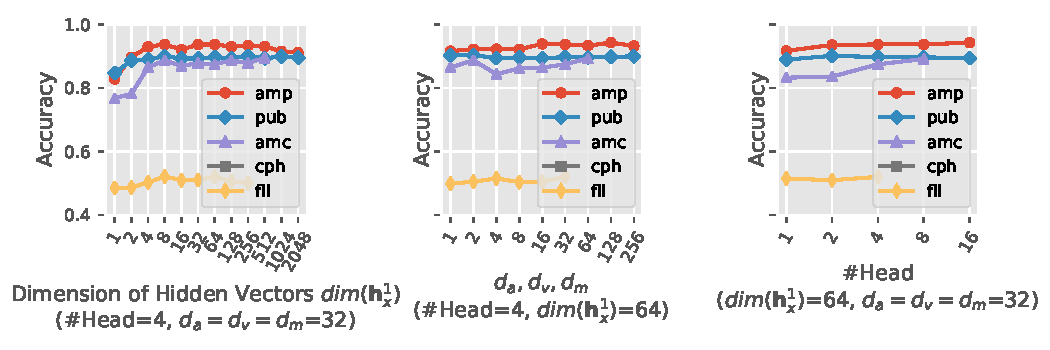
\includegraphics[width=1.0\columnwidth]{../figs/experiments/exp_hyperparameter_on_accuracy_gaan.pdf}
        \caption{Effects of hyper-parameters on accuracy of GaAN.}
        \label{fig:effect_of_hyper_parameter_on_accuracy_of_gaan}
   
    \end{figure}
   
    Second, the relative accuracy between the four GNNs varies greatly with different datasets.
    %
    There is no absolute winner.
    %
    We compare the best accuracy that each GNN achives on every dataset in Figure~\ref{fig:exp_hyperparameter_on_accuracy_alg_contrast}.
    %
    The best accuracy of the four GNNs are very close.
    %
    It is also close to the accuracy reported in [\cite{shchur2018_pitfall_of_gnn, zeng2020_graphsaint}].
    %
    GaAN that has the highest complexity performs slightly better than the other GNNs, winning three out of five datasets.
    %
    Simple GNN models (such as GCN) can still achieve good accuracy with proper hyper-parameter settings.
    
    \begin{figure}[h]
        \centering
        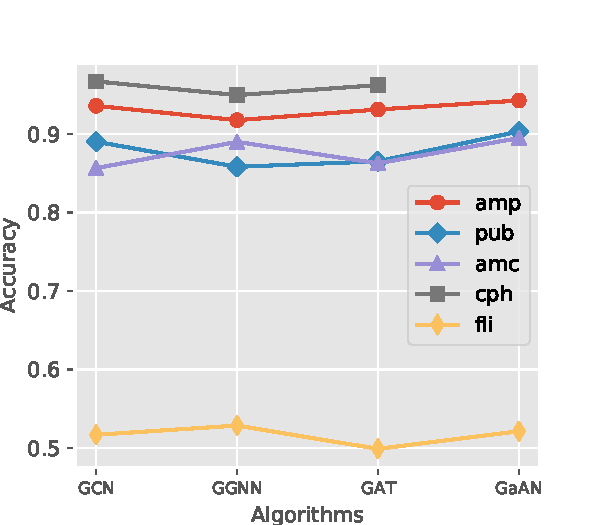
\includegraphics[width=3.5in]{../figs/experiments/exp_hyperparameter_on_accuracy_alg_contrast.pdf}
        \caption{Best accuracy that each GNN achieves on different datasets.}
        \label{fig:exp_hyperparameter_on_accuracy_alg_contrast}
    \end{figure}
    
    Besides, we add more details on the proportions of the train/evaluation/test sets of the datasets in Section 3.1 ``Experimental Setting'' in the revised manuscript.
    %
    Since the vertices of the \texttt{cam} dataset are not attached with feature vectors, we exclude it from the accuracy evaluation.
\end{reply}

\begin{point}
    Sampling method is definitely going to reduce model complexity, since all models complexity depend on graph node number N, while performance is going to be compromised as well. I would like to see authors resolve the concern of significant accuracy drop after applying aggressive sampling of subgraphs.
\end{point}

\begin{reply}

    Thanks for the insightful comment.
    %
    The sampling methods indeed affect the test accuracy of GNN models [\cite{hamilton2017_graphsage, chiang2019_cluster_gcn, zeng2020_graphsaint}].
    %
    %With or without the sampling methods, the structure of the GNN remains the same, but the gradients of the model parameters are calculated differently, affecting the accuracy of the GNN model.
    %
    %With sampling, each GNN layer still consists of $|\mathcal{V}|$ graph neurons ($|\mathcal{V}|$ is the number of vertices in the graph), but only graph neurons corresponding to the vertices in the sampled subgraph are activated.
    %
    %Thus, the model parameters are updated according to the gradients calculated on the sampled subgraph, instead of the whole graph.
    %
    %In other words, the GNN models are trained in a \emph{batch} gradient descent manner (i.e., full-batch training) without sampling.
    %
    %With sampling, the GNN models are trained with \emph{mini-bach} stochastic gradient descent.
    %
    To find out how the sampling techniques affect accuracy, we train the four typical GNNs with different batch sizes and compare the accuracy with the full-batch training.
    %
    For each combination of dataset and GNN, we use the hyper-parameters that achieve the highest accuracy under the full-batch training.
    %
    In most cases, the test accuracy of the sampling methods is just slightly lower than the accuracy of the full-batch training when the relative batch size $\geq 3\%$.
    %
    Among the two sampling methods, the performance of the cluster sampler is more stable than the neighbor sampler.
    %
    Figure~\ref{fig:exp_sampling_relative_batch_size_accuracy_graphsage} and Figure~\ref{fig:exp_sampling_relative_batch_size_accuracy_cluster} shows the accuracy of the two typical sampling methods under different batch sizes.
    %
    The results of the other datasets are available in Section 4.4.4 ``Effects on Accuracy'' in the revised manuscript.
    %
    In several cases (like GaAN in Figure~\ref{fig:exp_graphsage_sampling_accuracy_on_amp} and Figure~\ref{fig:exp_graphsage_sampling_accuracy_on_amc}), the accuracy of the neighbor sampler is even higher than the full-batch training.
    %
    The test accuracy of the cluster sampler is close to the accuracy of full-batch training, while the test accuracy of the neighbor sampler shows more obvious differences for different GNNs.
        

    \begin{figure}[h]
            \centering
            \subfloat[\texttt{amp}\label{fig:exp_graphsage_sampling_accuracy_on_amp}]{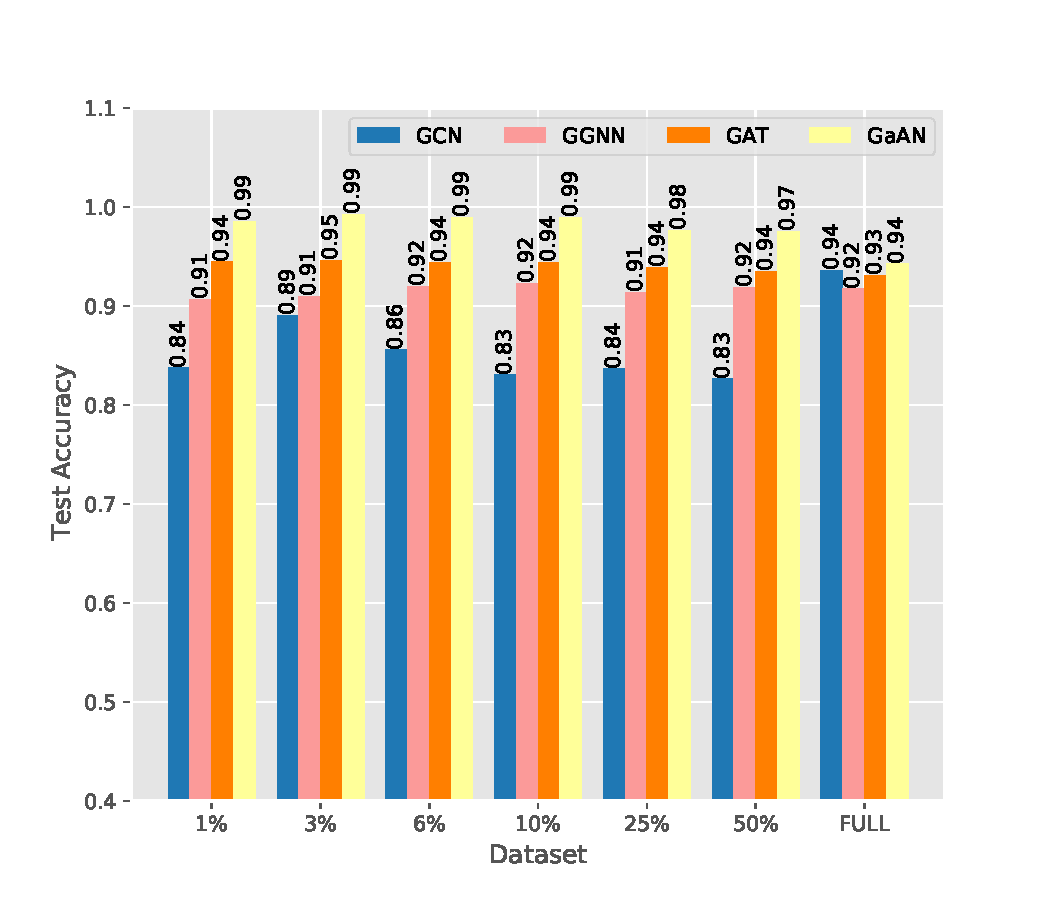
\includegraphics[width=0.33\columnwidth]{../figs/experiments/exp_graphsage_sampling_accuracy_on_amp.pdf}}
            \subfloat[\texttt{amc}\label{fig:exp_graphsage_sampling_accuracy_on_amc}]{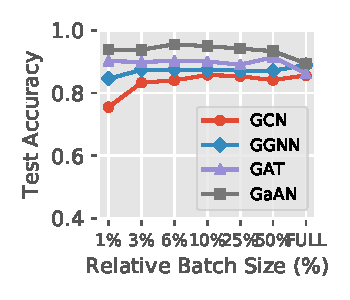
\includegraphics[width=0.33\columnwidth]{../figs/experiments/exp_graphsage_sampling_accuracy_on_amc.pdf}}
            \subfloat[\texttt{fli}\label{fig:exp_graphsage_sampling_accuracy_on_fli}]{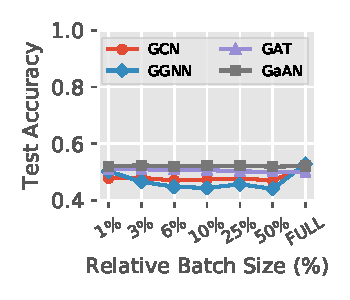
\includegraphics[width=0.33\columnwidth]{../figs/experiments/exp_graphsage_sampling_accuracy_on_fli.pdf}}
            \caption{Test accuracy of the neighbor sampler under different batch sizes. FULL means that the full graph participated in the training.}
            \label{fig:exp_sampling_relative_batch_size_accuracy_graphsage}
        \end{figure}
        
        \begin{figure}[h]
            \centering
            \subfloat[\texttt{amp}\label{fig:exp_cluster_sampling_accuracy_on_amp}]{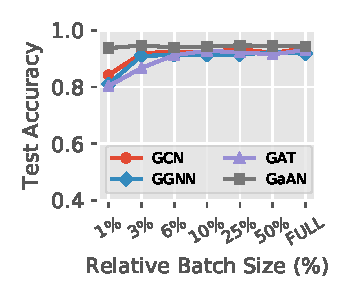
\includegraphics[width=2in]{../figs/experiments/exp_cluster_sampling_accuracy_on_amp.pdf}}
            %
            \subfloat[\texttt{amc}\label{fig:exp_cluster_sampling_accuracy_on_amc}]{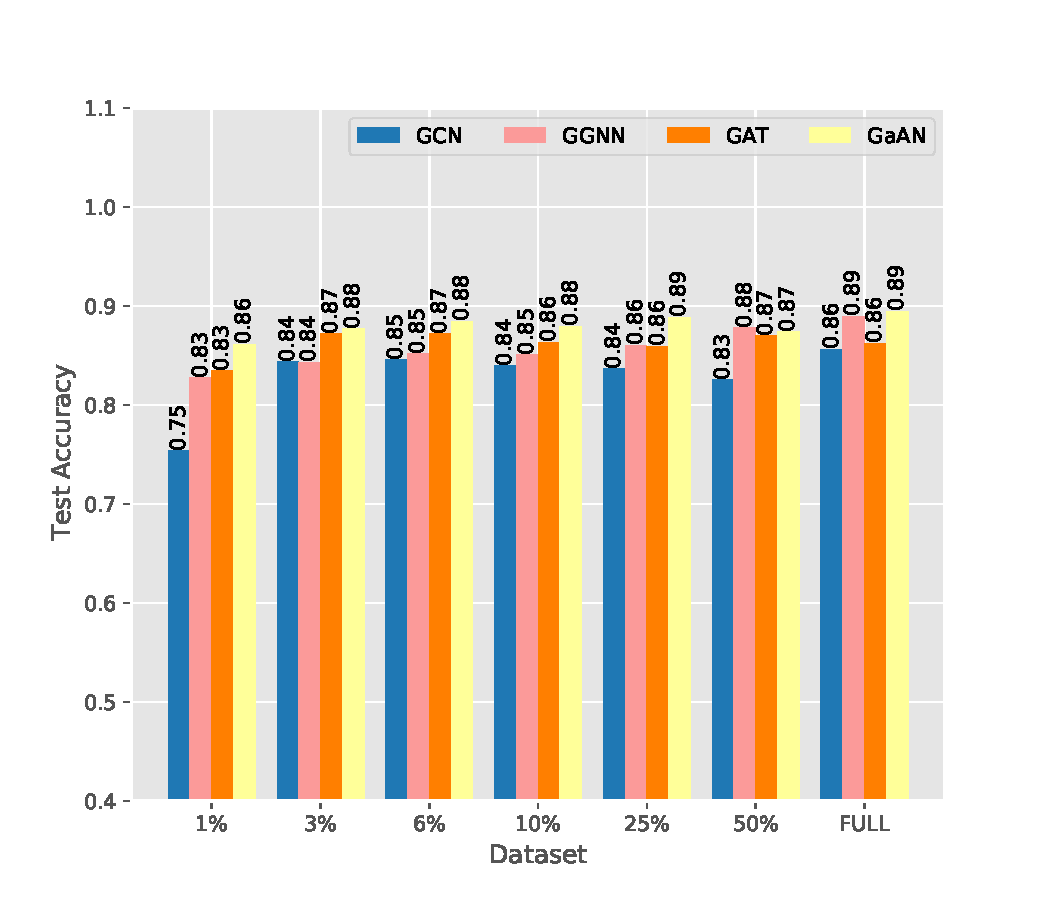
\includegraphics[width=2in]{../figs/experiments/exp_cluster_sampling_accuracy_on_amc.pdf}}
            %
            \subfloat[\texttt{fli}\label{fig:exp_cluster_sampling_accuracy_on_fli}]{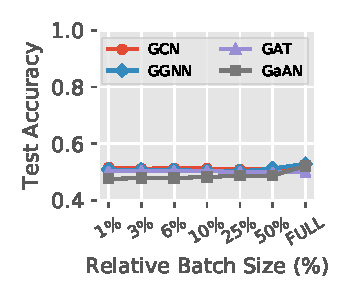
\includegraphics[width=2in]{../figs/experiments/exp_cluster_sampling_accuracy_on_fli.pdf}}
            \caption{Test accuracy of the cluster sampler under different batch sizes. FULL means that the full graph participated in the training.}
            \label{fig:exp_sampling_relative_batch_size_accuracy_cluster}
        \end{figure}
    
    The results indicate that the relationships between batch size and test accuracy are complex, especially for the neighbor sampler.
    %
    Larger batch size does not always bring higher accuracy, like GAT in Figure~\ref{fig:exp_graphsage_sampling_accuracy_on_fli}. 
    %
    Our observations are similar to [\cite{zeng2020_graphsaint}].
    %
    We believe that how to automatically select a proper batch size is a topic worth studying.
\end{reply}

\begin{point}
    Hope authors supplement the effect of sampling and GNNs on accuracy while comparing different complexity of model and sampling methods.
\end{point}

\begin{reply}

    We are grateful for your insightful suggestion.
    %
    Followed your suggestion, we additionally evaluate the effects of model complexity on accuracy in a new subsection Section 4.1.4 ``Effects on Accuracy'' in Section 4.1 ``Effects of Hyper-parameters on Performance''.
    %
    We add a discussion of how hyper-parameters of GNNs affect accuracy.
    %
    We also compare the test accuracy of different GNN models on the same dataset.
    
    We also additionally evaluate the effects of sampling techniques on accuracy in Section 4.4 ``Effects of Sampling Techniques'' in the revised manuscript.
    %
    We present the experimental results and related discussion in a new subsection Section 4.4.4 ``Effects on Accuracy''.
\end{reply}

\bibliographystyle{apalike}
\bibliography{../gnnref.bib}

\end{document}